\section{}
Recall the analog circuit from Assignment \#1

\begin{figure}[h]
    \centering
    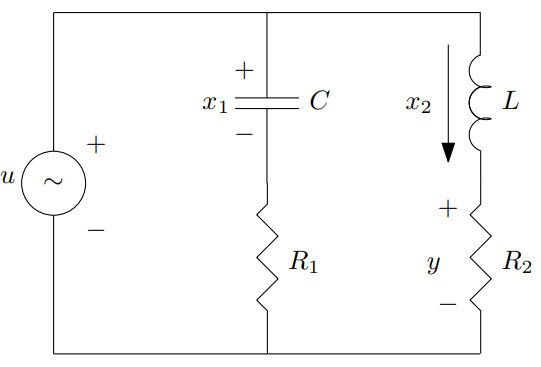
\includegraphics[width=0.5\textwidth]{Questions/Figures/Q3ProblemDiagram.png}
    \caption{Analog circuit from Assignment \#1}
    \label{fig:Q3ProblemDiagram}
\end{figure}

The input is the voltage $u$ and the response (output) is the voltage $y$. Find the transfer function
of this system

\begin{enumerate}[label=(\alph*)]
    \item Using the formula $G(s) = C(sI - A)^{-1}B + D$
    \item By applying the Laplace transform to the governing ODEs
\end{enumerate}

\textbf{Solution}\\
\subsection{}
From Assignment \#1, we have the state-space form
\begin{align*}
    A &= 
    \begin{bmatrix}
        -1/(R_1 C) & 0 \\
        0 & -R_2/L \\
    \end{bmatrix}, \;\;\;\;\;
    B =
    \begin{bmatrix}
        1/(R_1 C) \\
        1/L \\
    \end{bmatrix} \\
    C &=
    [0, R_2], \;\;\;\;\;
    D = 0
\end{align*}

By Matlab,
\begin{verbatim}
G =
 
R2/(R2 + L*s)
\end{verbatim}

Written nicely,
\begin{empheq}[box=\fbox]{align*}
    G(s) &= \frac{R_2}{R_2 + Ls}
\end{empheq}

This was given by the Matlab code:
\lstinputlisting[language=Matlab]{Questions/Code/a4q3.m}

\subsection{}
From the solution of Assignment \#1, we have the governing ODEs:
\begin{align*}
    \dot{x_2} &= -\frac{x_2}{L} + \frac{1}{L} u \\
    y &= R_2 x_2 \\
    \dot{y} &= R_2 \dot{x_2}
\end{align*}

Writing in terms of $y$,
\begin{align*}
    \frac{\dot{y}}{R_2} &= -\frac{y}{L} + \frac{1}{L} u \\
    \dot{y} &= -\frac{R_2}{L} y + \frac{R_2}{L} u
\end{align*}

Applying the Laplace transform to both sides,
\begin{align*}
    sY(s) - y(0) &= -\frac{R_2}{L} Y(s) + \frac{R_2}{L} U(s) \\
    (s + \frac{R_2}{L})Y(s) &= \frac{R_2}{L} U(s) + y(0) \\
    Y(s) &= \frac{R_2}{L(s + \frac{R_2}{L})} U(s) + \frac{y(0)}{s + \frac{R_2}{L}} \\
    &= \underbrace{\frac{R_2}{R_2 + Ls}}_{G(s)} U(s)} + \frac{y(0)}{s + \frac{R_2}{L}}
\end{align*}

By the definition of the transfer function,
\begin{empheq}[box=\fbox]{align*}
    G(s) &= \frac{R_2}{R_2 + Ls}
\end{empheq}

